% !TeX program = xelatex
\documentclass[UTF8,fontset=fandol,10pt,a4paper]{ctexart}
\usepackage[left=22mm,right=22mm,top=23mm,bottom=22mm,headheight=14pt]{geometry}
\usepackage{fontspec}
\setmainfont{TeX Gyre Heros}
\setsansfont{TeX Gyre Heros}
\setmonofont{Latin Modern Mono}
\renewcommand{\familydefault}{\sfdefault}
\usepackage[table]{xcolor}
\usepackage{graphicx,tikz}
\usetikzlibrary{arrows.meta,positioning,fit,backgrounds,calc}
\usepackage{booktabs,tabularx,array,enumitem,float,caption,fancyhdr,hyperref}
\definecolor{blue}{HTML}{2869A9}
\definecolor{ink}{HTML}{293340}
\definecolor{muted}{HTML}{647181}
\definecolor{line}{HTML}{C5D4E2}
\definecolor{pale}{HTML}{F0F5FA}
\definecolor{warm}{HTML}{FFF7E9}
\hypersetup{colorlinks=true,urlcolor=blue,linkcolor=blue,pdftitle={Redflag RHI 与 Vulkan 接入设计},pdfauthor={Redflag}}
\color{ink}
\setlength{\parindent}{0pt}
\setlength{\parskip}{6pt}
\linespread{1.16}
\setlist[itemize]{leftmargin=1.5em,itemsep=2pt,topsep=3pt}
\setlist[enumerate]{leftmargin=1.8em,itemsep=3pt,topsep=3pt}
\renewcommand{\arraystretch}{1.38}
\newcolumntype{Y}{>{\raggedright\arraybackslash}X}
\newcolumntype{L}[1]{>{\raggedright\arraybackslash}p{#1}}
\ctexset{section={format=\Large\bfseries\color{blue},beforeskip=16pt,afterskip=8pt},subsection={format=\large\bfseries\color{blue},beforeskip=11pt,afterskip=5pt}}
\captionsetup{font=small,labelfont=bf,textfont={color=muted},skip=7pt}
\pagestyle{fancy}\fancyhf{}
\fancyhead[L]{\small\color{muted}Redflag · RHI / Vulkan · 设计方案}
\fancyhead[R]{\small\color{muted}2026-11-21}
\fancyfoot[C]{\small\color{muted}\thepage}
\renewcommand{\headrulewidth}{0pt}
\newcommand{\note}[1]{{\small\color{muted}#1\par}}
\newcommand{\code}[1]{{\small\texttt{#1}}}
\newcommand{\ruleline}{\par\vspace{4pt}{\color{line}\hrule}\vspace{8pt}}
\newcommand{\source}[2]{{\small\href{#1}{[#2]}}}
\tikzset{
 module/.style={draw=line,fill=pale,rounded corners=2pt,align=center,inner sep=7pt,text width=3.8cm,minimum height=1.15cm,font=\small},
 smallbox/.style={module,text width=2.55cm,minimum height=.95cm,font=\footnotesize},
 wide/.style={module,text width=9.5cm},
 planned/.style={module,fill=warm,dashed},
 flow/.style={-{Stealth[length=2mm]},draw=muted,line width=.65pt},
 own/.style={flow,dashed},
 label/.style={font=\scriptsize,fill=white,inner sep=2pt,text=muted}}

\hypersetup{pdftitle={Redflag 经典场景实测}}
\fancyhead[L]{\small\color{muted}Redflag · 经典场景}
\graphicspath{{../../../output/scenes/}}
\begin{document}
\zihao{5}\raggedright
\setlength{\parindent}{2\ccwd}
\ctexset{section={afterindent=true}}
{\Huge\bfseries 经典场景实测}\par
{\large\color{muted}Cornell Box、Sponza 中庭与 Sun Temple}\par
\ruleline

\section{Cornell Box 的红墙与白盒}
先从开口正面看房间。左墙是红色，右墙是绿色，中间的两个方块和地面都用白色材质。在红墙旁的白地板和高块侧面可以看到浅红色。左后高块和右前矮块的轮廓分得开，方块背光面比朝光面暗。顶面有一处亮斑，后墙与顶面接缝处也能看到细亮线。换后端后可以从同一相机位置检查这些位置有没有变化。
\begin{center}
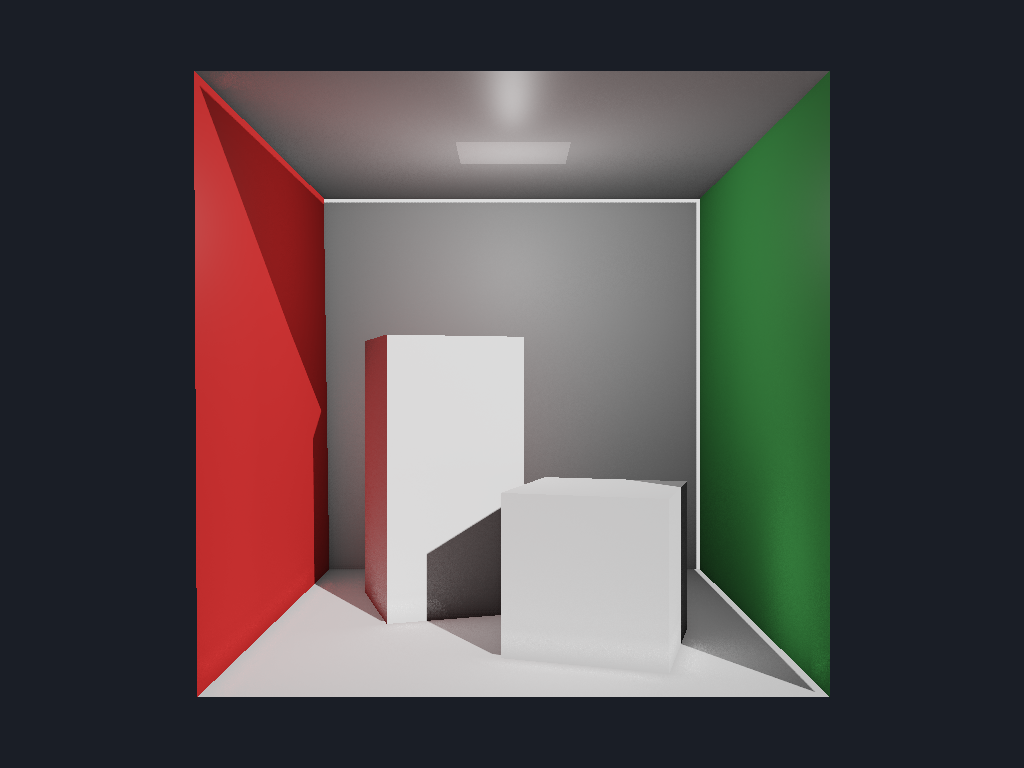
\includegraphics[width=.90\linewidth]{CornellBox.png}
\end{center}
方向光沿 $(-0.6,-0.6,-1)$ 从前方斜照红墙。反射阴影图（RSM）根据这堵墙收到的光，估算它又给附近白地板送去多少光。本次把这个效果的强度设为 1。另有一盏点光源参与直接光照。天花板上的白色矩形是模型几何，编辑器中的点光源单独放置。所以可以用这幅图检查方块的位置和遮挡，或比较同一块地板上的反光。要与 Cornell 的实测照片比较，还需要对应面光源和测量过的反射率。

为了下次还能找到同一块地面，测试固定了模型和相机。模型最长边缩放到 4 个场景单位。相机位于 $(0,0,7.8)$，看向原点，垂直视场角 $45^\circ$。分辨率 $1024\times768$，曝光为 1，开启屏幕空间环境遮蔽与反射阴影图，取连续绘制的第 12 帧。5 个子网格共 32 个三角形，397,212 个像素写入了模型的实体编号。

\source{https://bowers.cornell.edu/cornell-box}{Cornell University 原实验}
\quad\source{https://github.com/nvpro-samples/vk_mini_path_tracer/blob/9d6a0e4242790ddac52a0d8ee02eb7670bf10965/scenes/readme.txt}{Cardenas 与 McGuire 的几何数据，CC BY 3.0}
\note{项目保留原顶点、法线和面，为两侧墙体、白色物体和顶灯片补了实时渲染用的 RGB 材质。图像取自 Redflag 的最终颜色纹理。}

\newpage
\section{白地板上的反射光}
保持第一页的相机、灯光和曝光，分别关闭和开启反射阴影图，每次都取第 12 帧。左图关闭反射光，右图将它加回房间。中图把右图比左图多出的光单独显示，靠近红墙的地面最容易看清。中图的显示倍率见图内标注。下表直接比较线性 HDR 颜色，数值不经过曝光、色调映射或截图取色。
\begin{center}
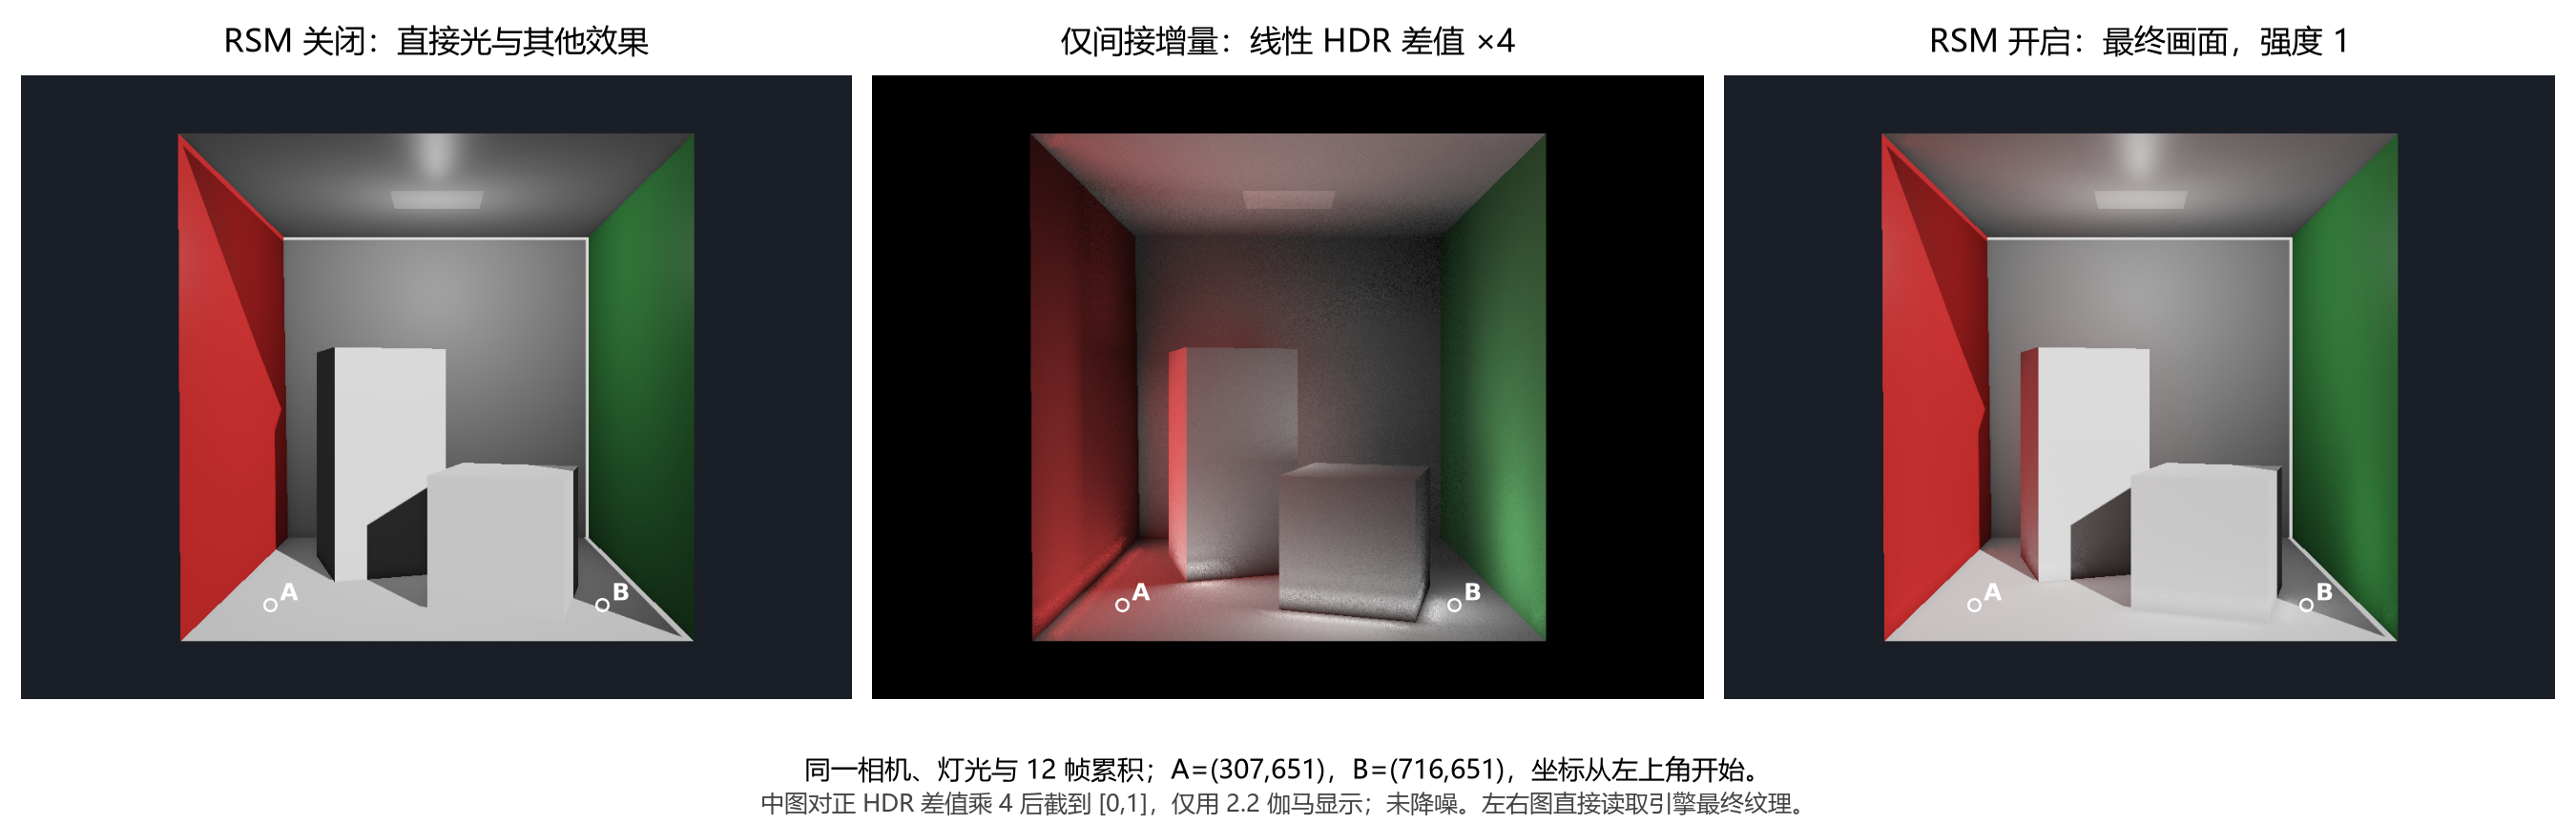
\includegraphics[width=\linewidth]{rsm/Cornell-RSM.png}
\end{center}

对照点在白色地板上。按图像左上角为原点，它位于 $(307,651)$，靠近红墙。设 $\Delta C=C_{\rm on}-C_{\rm off}$。同一灯光与强度下，$\Delta R$ 大于 $\Delta G$ 和 $\Delta B$，表示地面因反射光变红。
\begin{center}
\begin{tabular}{lrrr}\toprule
斜照红墙 & $\Delta R$ & $\Delta G$ & $\Delta B$ \\ \midrule
修正前，强度 5 & 0.07715 & 0.03076 & 0.03076 \\
修正后，强度 5 & 0.48218 & 0.13550 & 0.13550 \\
最终场景，强度 1 & 0.09644 & 0.02710 & 0.02710 \\ \bottomrule
\end{tabular}
\end{center}
先对照表格的前两行。它们用相同强度，红色通道从 0.07715 增加到 0.48218，说明变化来自算法。第三行才是第一页画面采用的强度。旧版原场景方向光朝向绿墙时，光源看到的红墙没有收到这盏灯的正面照明，红墙反射通量为零；增加强度也无法把这些采样点变红。点光源只参与直接光照。

独立的两面片场景只留下红色反射面和白色接收面，消除了其他白墙的影响。在相同强度 1 下，白面上选点的红色增量从 0.05371 变为 0.15186。数学推导和源码对照见《渲染公式与实现》。本例估算一次漫反射，没有测量真实房间的反射率，也没有计算从反射点到接收点之间的逐点遮挡。

\newpage
\section{Sponza 的石柱与织物}
在 Cornell Box 中，几块色面就够看清光线的变化。接下来换到 Sponza，检查导入许多不同材质以后，引擎能否把每张贴图用在正确的位置。沿中庭望去，两排石柱和拱券之间挂着红、蓝、绿三种织物。近处垂布可以看到褶皱和金色纹样，远端石墙仍有层次。画面中个别织物和墙面有较亮的斑点。这次记录了现象，成因需要用固定相机分别关闭法线贴图、间接光等效果再检查。
\begin{center}
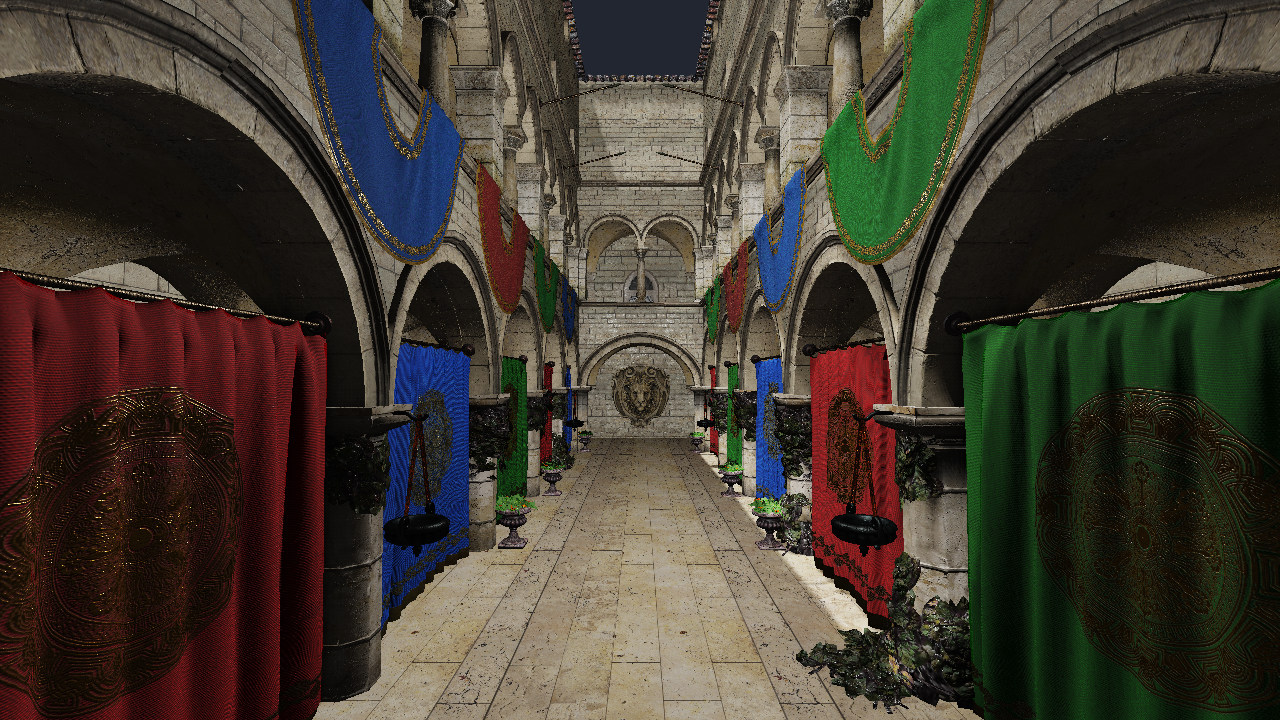
\includegraphics[width=\linewidth]{Sponza.png}
\end{center}
第一次取景时只用方向光，入口拱下的布料偏暗。最终相机移到 $(-5.5,-2.2,0)$，朝向 $(6,-1.8,0)$，垂直视场角 $65^\circ$。在 $(-2,-1,0)$ 补一盏强度 2、半径 20 的点光，把曝光设为 1.4。这个构图用来观察凹槽和织物细节。

在 $1280\times720$ 的画面上，测试开启屏幕空间环境遮蔽和反射阴影图。模型由 103 个子网格组成，从这台相机看有 21 个落在视野外，主画面跳过了它们。本帧 Renderer3D 统计到 372 次绘制，912,256 个像素写有模型编号。最终颜色取第 12 帧，取图时检查了色调映射前的每个颜色值，均为有限数。

本例采用 Khronos 发布的 Crytek Sponza glTF 版本。原始建筑模型由 Marko Dabrović 制作，Crytek 版本由 Frank Meinl 重制。下载脚本固定上游版本，读取模型文件列出的几何数据和 69 张图像。完整模型与贴图保存在本机。仓库附有场景、取图时的设置、实测图，以及下一页所用的下载脚本。

\source{https://github.com/KhronosGroup/glTF-Sample-Assets/blob/e124e8d8d7330a5372bc2b4d00d39a4a9d7997ea/Models/Sponza/README.md}{模型来源与版本说明}
\quad\source{https://github.com/KhronosGroup/glTF-Sample-Assets/blob/e124e8d8d7330a5372bc2b4d00d39a4a9d7997ea/Models/Sponza/LICENSE.md}{资产许可}

\newpage
\section{场景加载与截帧回放}
要从编辑器重看这两张图，从 Forge 打开 \path{assets/scenes/Reference-CornellBox.redflag} 或 \path{assets/scenes/Reference-Sponza.redflag}，运行场景后使用保存的主相机。Cornell Box 的几何随仓库提供；Sponza 首次运行前在仓库根目录执行下载脚本。灯光与模型保存在场景文件里，实测用的后处理开关和尺寸见对应 YAML。

以下命令均从仓库根目录运行。第一行准备 Sponza，后两行按各自的 YAML 绘制并保存场景图。
\begin{verbatim}
python tests/fetch_sponza.py
tests\run_scene_gallery.cmd tests\scenes\cornell.yaml
tests\run_scene_gallery.cmd tests\scenes\sponza.yaml
\end{verbatim}

上面的命令会先加载模型，把模型、灯光和相机保存成编辑器可以打开的场景，再重新读回并绘制。这也检查了保存以后，模型路径和相机位置是否还能正确还原。每帧先写主渲染目标，后处理得到最终颜色。程序从该纹理读回像素，按 PNG 的图像方向翻转行。两张图均在 Debug/x64、GeForce RTX 5070 Ti Laptop GPU、OpenGL 4.6、NVIDIA 616.56 上生成。

拿到图以后，先在盒子内部读一个实体编号，再读背景。前者应指向模型，后者应为 $-1$。接着检查浮点颜色里是否出现无效数值。这两项能发现空画面和部分计算错误。材质色差、法线方向、阴影边缘仍需结合可见画面检查。每次实测的设备、像素数和绘制统计保存在 \path{output/scenes/} 中与图像同名的 YAML。

如果几何和颜色对不上，可以直接回放 Cornell Box 的第 12 帧。它保存在 \path{output/scenes/CornellBox_capture.rdc}。RenderDoc 1.47 在回放中以附件格式、颜色写入开关和索引数核对了阴影、反射阴影图、深度预写与主绘制。每个阶段绘制 5 个子网格，共 96 个索引。整帧有 24 次绘制，包含全屏处理；它与 Renderer3D 自身统计的 22 次口径不同。

最后一次绘制为事件 273。导出的 $1024\times768$ 颜色图与运行时读回图逐像素比较，三个 RGB 通道完全一致。捕获时驱动报告了 9 条缓冲性能提示和 6 条着色器状态重编译提示。开启验证后的回放新增 12 条信息，最终状态为 Success。本例没有采 GPU 时间，这些提示没有对应的耗时结论。事件和消息可在 \path{output/scenes/CornellBox-replay.json} 查到。

\note{渲染公式与关键源码见《渲染公式与实现》。排查透明裁剪和着色器链接错误的旧代码、修改与验证见《排错记录》。}
\clearpage
\fancyhead[R]{\small\color{muted}Vulkan · Sponza}
\section{中庭雕塑展}
主相机朝着中庭的长廊。玉绿色的龙占据画面中央，两侧分别放了赤陶色的兔子和赭色的佛像。三件雕塑采用 Stanford 的扫描网格，台座则直接用引擎的立方体。模型尺寸各不相同，摆放时先将它们缩放到想要的高度，再将各自最低的顶点移到台面。这样改龙的大小时，它的脚还能落回原处。

\begin{figure}[H]\centering
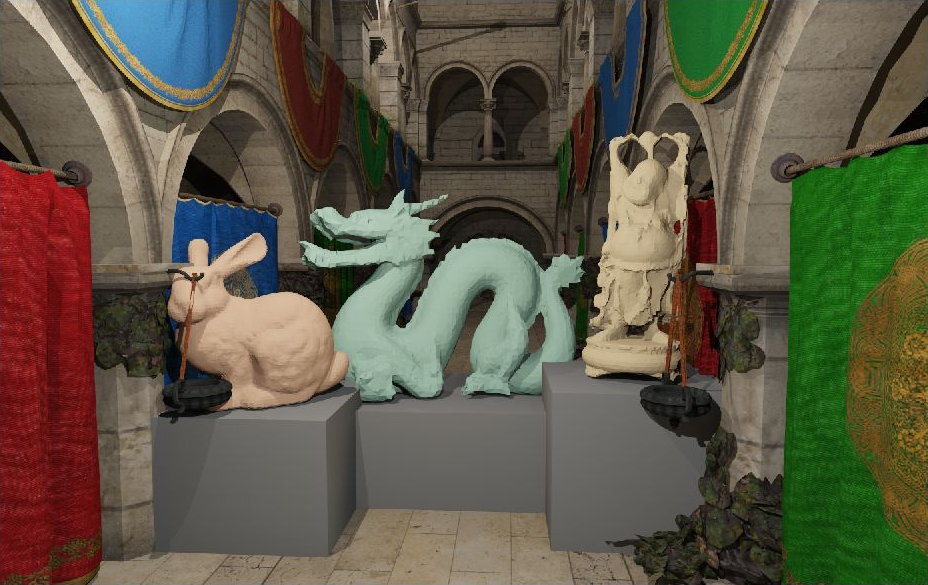
\includegraphics[width=.96\linewidth]{Sponza-Sculpture-Gallery.png}
\caption{RedflagForge 实际 Game 视口。展品的摆放、材质底色、灯光和机位保存在场景文件中。}
\end{figure}

要接着布光，先在主相机视图看一眼龙的轮廓，再回到场景视图选「主灯」。这盏暖色点光源从前侧照向雕塑。另一侧的冷光把龙的头颈从深色布景中分出来。镜头前还有一盏名为「补光灯」的点光源，降低它的强度可以看到龙身凹处的阴影加深。主相机留在原处，在两个视图之间切换，能看清移灯究竟改变了雕塑的哪一面。保留机位，在「实时效果」勾选「对照：只显示直接光」，还可以单独看灯直射到的部分，取消勾选即可看回完整光照。

资源准备好后，在项目面板双击 \path{Sponza-Sculpture-Gallery.redflag}。首次在新机器上打开时，从仓库根目录分别运行 \path{python tests/fetch_sponza.py} 与 \path{python tests/fetch_stanford.py}。原始网格和纹理按各模型的来源及使用条件提供，场景文件只保存对模型的引用。
\par\noindent
\source{https://graphics.stanford.edu/data/3Dscanrep/}{Stanford 扫描模型}
\quad\source{https://github.com/KhronosGroup/glTF-Sample-Assets/tree/main/Models/Sponza}{Khronos · Sponza 模型与许可}

\clearpage
\fancyhead[R]{\small\color{muted}Vulkan · Sun Temple}
\section{神庙长廊}
入口两旁的雕像背对廊灯，翅膀边缘比身体亮。沿地面的红色镶边向里看，石柱从偏暖的浅灰逐渐过渡到冷灰。这里保留了 Epic Games 随模型提供的入口机位，布光则在 Redflag 中重新安排。前厅和长廊各有自己的点光源，调整其中一盏，就能在这条连续的地面上看到影响范围。

\begin{figure}[H]\centering
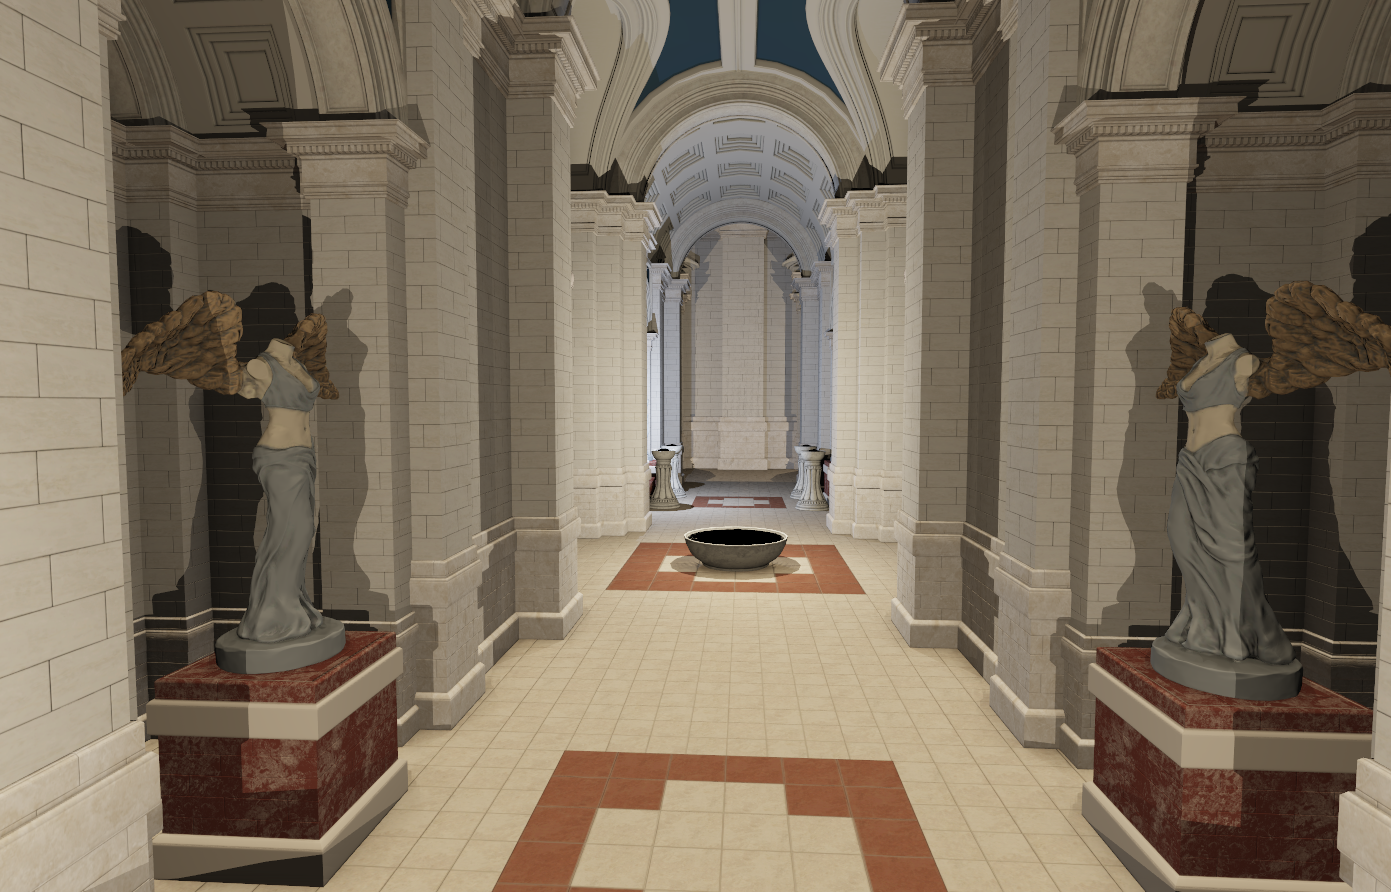
\includegraphics[width=.96\linewidth]{sun-temple/SunTemple.png}
\caption{Redflag 的 Vulkan 视口，第 12 帧。图中使用全部八盏点光源，以及 DDGI、GTAO 和 TAA。场景原图为 $1391\times892$ 像素，从编辑器实际提交给 ImGui 的图像导出。}
\end{figure}

第一次打开前，在仓库根目录运行 \path{python tests/fetch_sun_temple.py}。脚本需要 Blender 5、Pillow 和 NumPy。它检查原始压缩包，把静态建筑变成编辑器能加载的 glTF，再把 DDS 贴图转换为 PNG。回到编辑器，在项目面板双击 \path{Sun-Temple.redflag}。选中「前厅灯」调低强度，雕像旁的地砖会先暗下去，长廊后半段仍受另外几盏灯照亮。想保留这个改动，保存场景即可。

原始模型包含 517 件静态物体。它们仍保持各自的位置；为了减少重复加载相同材质，准备脚本按材质将几何合为 48 组，共 606,376 个三角形。这批模型和图像来自 Epic Games，由 Kai-Hwa Yao 与 Nicholas Hull 从 Unreal Engine 导出并发布在 NVIDIA ORCA，许可为 CC BY-NC-SA 4.0。

\par\noindent\source{https://developer.nvidia.com/ue4-sun-temple}{NVIDIA ORCA · Sun Temple}
\quad\source{https://creativecommons.org/licenses/by-nc-sa/4.0/}{模型与配图许可}
\quad\href{run:../scenes/sun-temple/README.md}{导入方法与截帧记录}

\clearpage
\section{火盆上的余烬}
走近神庙墙角的火盆，盆沿和石柱都受房间里的灯照亮。盆里的炭也有自己的颜色。模型给它附了一张自发光贴图，只有细小的炭纹发红。旧版导入了火盆，却漏读了这张图，所以房间的灯再亮，盆中也少了这层红色。

\begin{figure}[H]\centering
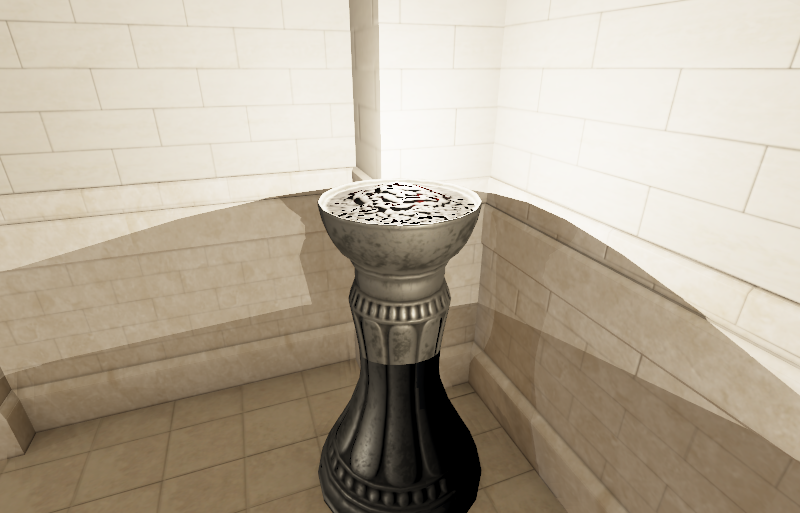
\includegraphics[width=.75\linewidth]{../../../output/profiling/emissive-studio/temple.png}\\[5pt]
\begin{minipage}{.47\linewidth}\centering
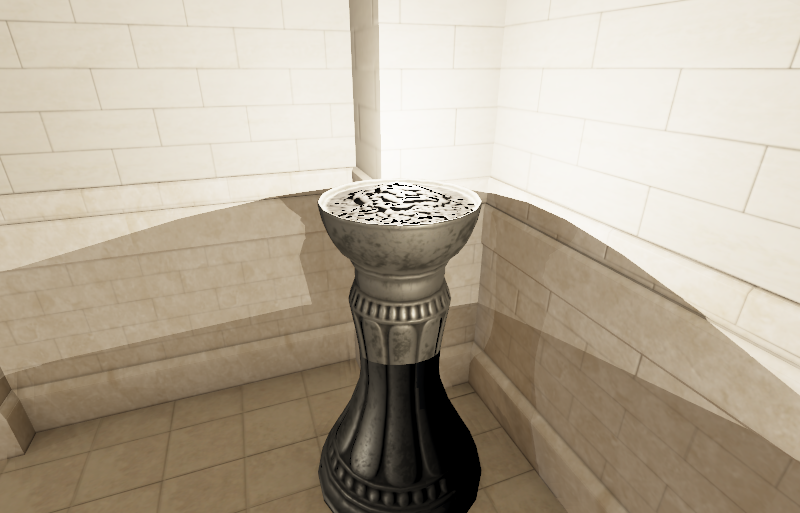
\includegraphics[width=\linewidth,trim=310bp 278bp 310bp 172bp,clip]{../../../output/profiling/emissive-studio/temple-before.png}\\旧版\end{minipage}\hfill
\begin{minipage}{.47\linewidth}\centering
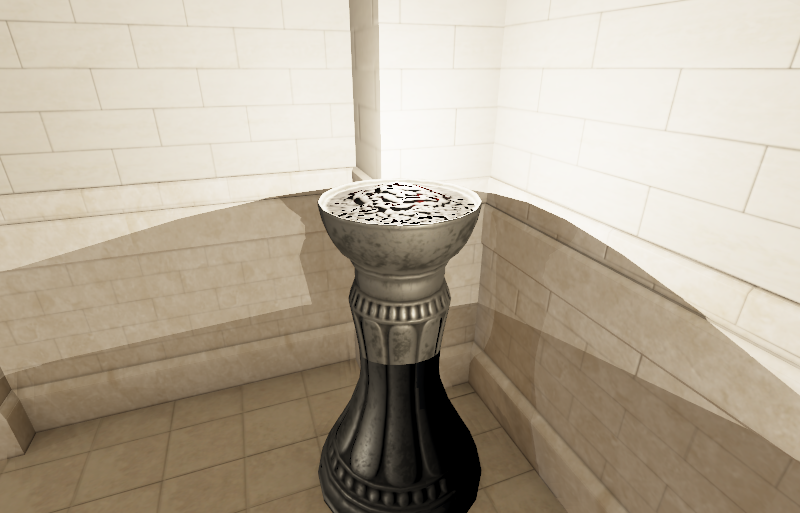
\includegraphics[width=\linewidth,trim=310bp 278bp 310bp 172bp,clip]{../../../output/profiling/emissive-studio/temple.png}\\读入自发光以后\end{minipage}
\caption{上图是 Redflag Vulkan 编辑器中的火盆。下排放大同一块盆面，保留编辑器原来的颜色。两次截帧使用同一机位、同一组灯和相同的曝光。}
\end{figure}

最明显的一处在原图坐标 $(419,202)$，从左上角开始计数。显示器还没有调整亮度时，这里的红色从 0.274 增至 0.878，绿色只从 0.214 变为 0.216。整张图中，红色增量超过 0.1 的只有 104 个像素。因此比较这种细小材质时，要把盆面放大，并读回原来的颜色。整幅画面的平均亮度很难告诉我们炭纹有没有画出来。

\source{https://developer.nvidia.com/ue4-sun-temple}{模型与贴图：Epic Games / NVIDIA ORCA}
\quad\href{run:../profiling/emissive-studio/README.md}{相机、截帧与测量方法}

\end{document}
